\section{Diode und Kennlinien}
Ziel dieses Versuchs ist es, die Arbeitsweise der Diode besser n\"aher zu bringen und das erworbene Wissen aus der Theorie zu vertiefen. 
\subsection{Experimentelle Durchf\"uhrung}
Zun\"achst wird die Schaltung wie in der Abbildung 1 auf dem Steckbrett aufgebaut. Dazu wird ein Widerstand R$_1$ $=$ 1~$k\Omega$ ben\"otigt. Als Messwiderstand wird ein Widerstand R$_2$ = 100~$\Omega$ verwendet, um den Diodenstrom bestimmen zu k\"onnen. Als Eingangspannung wird eine sinusf\"ormige Spannungsquelle U$_{ein_{pp}}$ = 5~$V$ angelegt. Um die Strom-Spannungskennlinien der Dioden zu bestimmen, wird der Spannungsabfall an dem \textbf{X-Kanal} und \textbf{Y-Kanal} gemessen. Der Versuch wird analog f\"ur alle drei Dioden durchgeführt(siehe Tabelle 1). \\
Anschlie\ss end wird der differentielle Widerstand der \textbf{Si-Diode} bei 0.7~$V$ bestimmt. Als n\"achstes wird die gleiche \textbf{Si-Diode} mit einem Eisspray abgek\"ult und die angezeigte Kennlinie mit der Kennlinie bei Raumtemperatur verglichen. Au\ss erdem wird die Diodenspannung der gek\"ulten Diode ermittelt. 
\begin{figure}[ht]
\begin{center}
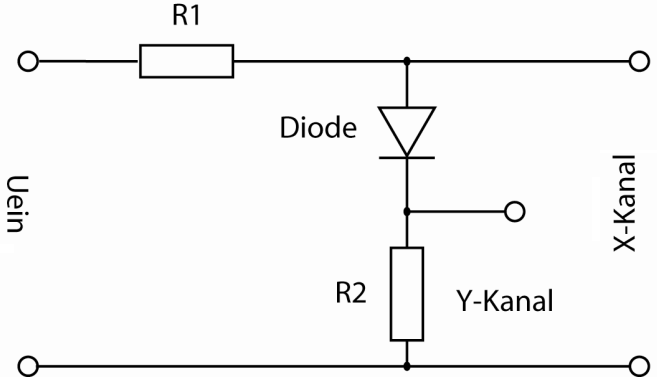
\includegraphics[scale=0.4]{schaltungVersuch1}
\caption{Schaltung zur Aufnahme der Diodenkennlinie}
\end{center}
\end{figure}

\begin{table}[ht]
\begin{center}

\caption{Dioden Typen}
\begin{tabular}{|l|l|}
\hline
Messreihe & Diodentyp \\
\hline
1 & Si-Universal-Diode \textbf{1N4148} \\
\hline
2 & Schottky-Diode \textbf{BAT41} \\
\hline
3 & Z-Diode \textbf{ZPD2,4} oder \textbf{ZF2,4} \\
\hline
\end{tabular}
\end{center}

\end{table}

\subsection{Ergebnisse und Diskussion}
Die Strom-Spannungskennlinie wird mit Hilfe der \textbf{XY-Funktion} des Oszilloskops angezeigt. Die Dioden Verl\"aufe sind mit dem Einsetzen eine Sinusf\"ormige Wechselspannung und eine Frequenz von ca. 100$Hz$ (also ein nicht so gro\ss e Frequenz) erwiesen sich als sinnvoll, da der Anstieg der Spannung m\"oglicht stetig sein sollte, und damit eine besser Strom-Spannungsverl\"aufe dargestellt werden k\"onnen.    \\
Die abgek\"ulte Diode hat eine h\"ohre Durchlassspannung als die selbe Diode unter Normalbedingungen. \\
Mittels der in der Vorbereitung gegebenen Formel wird die neue Temperatur bestimmt.
\begin{figure}[!h]
\begin{minipage}{0.4\textwidth}
\begin{center}
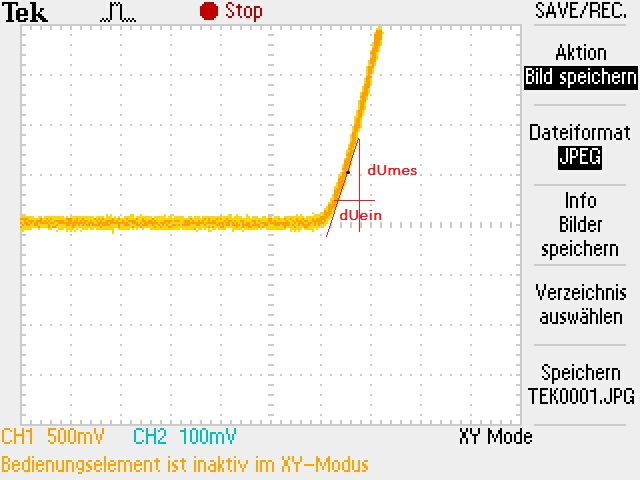
\includegraphics[scale=0.6]{bilder/Versuch2/siDiode}
\caption{Strom-Spannungskennlinie \textbf{Si-Diode}}
\end{center}
\end{minipage}
\hfill
\begin{minipage}{0.4\textwidth}
\begin{center}
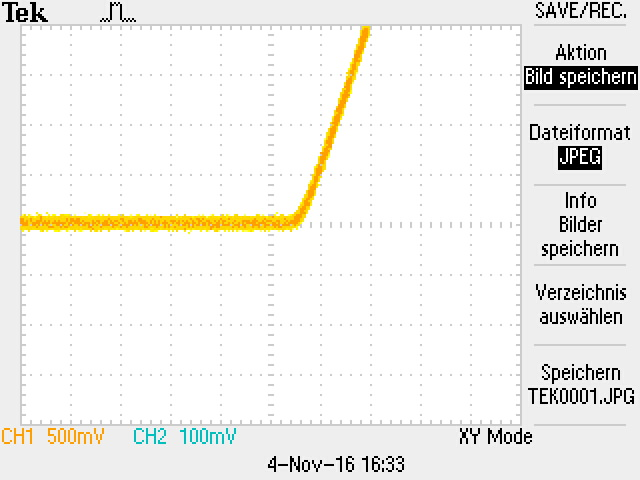
\includegraphics[scale=0.6]{bilder/Versuch2/SchottkyDiode}
\caption{Strom-Spannungskennlinie \textbf{Schottky-Diode}}
\end{center}
\end{minipage}
\end{figure}
\begin{figure}[!h]
\begin{center}
\begin{minipage}{0.4\textwidth}
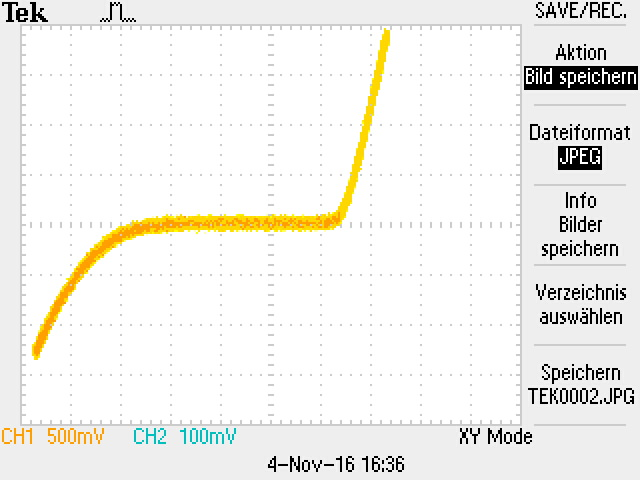
\includegraphics[scale=0.6]{bilder/Versuch2/zDiode}
\caption{Strom-Spannungskennlinie \textbf{Z-Diode}}
\end{minipage}
\end{center}
\end{figure}
\noindent
Man kann deutlich erkennen, dass bei der \textbf{Si-Diode} kein Strom flie\ss t, wenn die Eingangsspannung die Schwellenspannung der Diode nicht \"ubersteigt. Sofern die Spannung die Schwellenspannung \"ubersteigt, kommt es zu ejnem schnellen Anstieg des Stroms. Bei einer \textbf{Schottky-Diode} ist das gleiche Verhalten wie bei einer \textbf{Si-Diode} zu erkenen, au\ss er, dass die Schwellenspannung der \textbf{Schottky-Diode} kleiner ist als der der \textbf{Si-Diode}. Bei der \textbf{Z-Diode} ist zus\"atzlich noch die Durchbruchspannung zu erkennen, bei der, der Strom eine \"Anderung in negativer Richtung hat.
\\ 
\begin{equation*}
r =\frac{\Delta U}{\Delta I} = \frac{\Delta U}{\Delta U_{mess}} \cdot R_2 = 214 \Omega 
\end{equation*}
Der Wert der differentiellen Widerstand ist zu Vergleich mit dem Wert der Berechnung ziemlich gr\"o\ss, das kann man erkl\"aren, dass der Messwiederstand in der Berechnung nicht ber\"ucksichtigt w\"urde.\\ 
In der Abbildung 5 ist der Spannungsverlauf der gek\"uhlten \textbf{Si-Diode} dargestellt. Es ist zu erkennen, dass die Schwellenspannung h\"oher liegt als die der ungek\"uhlten \textbf{Si-Diode}. Die Temperatur der gek\"uhlten \textbf{Si-Diode} liegt bei ca. 10$^\circ$.
\begin{figure}[!h]
\begin{center}
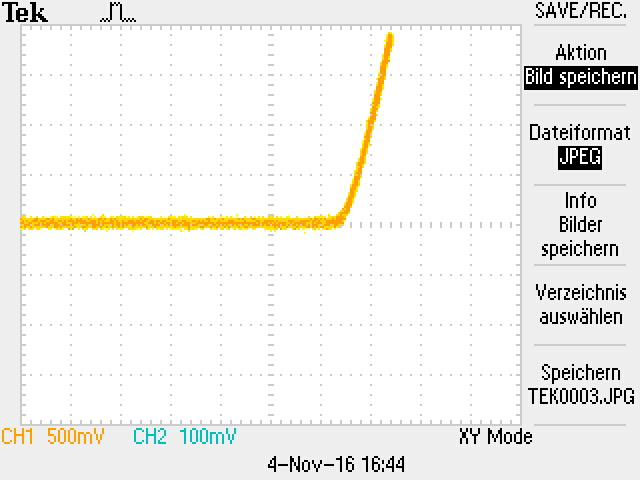
\includegraphics[scale=1]{bilder/Versuch2/kuhlsiDiode}
\caption{Strom-Spannungskennline der gek\"ulten \textbf{Si-Diode}}
\end{center}
\end{figure}